\chapter{Experiments and Results}
\label{chap:impl}

This chapter presents a comprehensive examination of various experiments designed to investigate the effectiveness of knowledge distillation techniques in enhancing the performance of smaller models through the utilization of LLM\@.

The experiments are systematically structured to compare baseline models, explore innovative architectural modifications, and assess the impact of training strategies on model accuracy and efficiency in sequence classification tasks. The experimental findings are crucial for validating the theoretical propositions discussed in previous chapters and for demonstrating the practical capabilities of distillation methodologies in real-world applications.

Additionally, this chapter aim to deepen the understanding of knowledge distillation processes and their practical applications in enhancing the efficacy of smaller models by leveraging the knowledge embedded within LLM\@. The results from these experiments will provide valuable insights that could reshape approaches to model training and optimization in the field of NLP\@.

\newcounter{experiment}
\stepcounter{experiment}
\section{Experiment \theexperiment: Evaluating the baselines}

In this section, I detail the methodologies and results of the experiment aimed at evaluating the baseline models described in \autoref{sec:baselines}. The primary goal of this experiment is to assess the performance of each model across datasets provided in \autoref{sec:datasets} to establish a benchmark for future comparative analyses.

\subsection*{Experimental Setup}

Prior to the training process, the datasets were segmented into smaller portions (\autoref{tab:dataset_portions}). The rationale behind selecting varied dataset sizes, including smaller subsets and relatively larger subsets, is to enable a more precise evaluation of model distillation techniques across different scales of data. This approach allows for a detailed comparison of how data volume impacts the effectiveness of distillation in transferring knowledge from larger to smaller models. This standardized approach is crucial for mitigating variability in dataset size, which can influence the accuracy and reliability of the results, particularly when assessing model performance under different data constraints.

\begin{table}[h]
    \centering
    \caption{Number of samples in each dataset portion}
    \label{tab:dataset_portions}
    \resizebox{\textwidth}{!}{
        \begin{tabular}{lccccccccc}
            \toprule
                                         & \multicolumn{9}{c}{\textbf{Portion size}}                                                                                                                            \\
            \textbf{Dataset}             & \textbf{0.01}                             & \textbf{0.03} & \textbf{0.05} & \textbf{0.07} & \textbf{0.1} & \textbf{0.3} & \textbf{0.5} & \textbf{0.7} & \textbf{1.0} \\

            \midrule
            WOS (\autoref{sec:wos})      & N/A                                       & N/A           & N/A           & N/A           & 380          & 1,138        & 1,896        & 2,654        & 3,791        \\
            e-SNLI (\autoref{sec:esnli}) & 386                                       & 1,156         & 1,926         & 2,697         & 3,852        & 11,556       & 19,260       & 26,964       & 38,520       \\
            \bottomrule
        \end{tabular}
    }
\end{table}

Each model was trained on the datasets using a predefined split of training and validation data, same for each model. Model validation was performed intermittently during training to monitor performance, adjust parameters as necessary and use early stopping to prevent overfitting.

After training, each model was evaluated on a separate test set that was not used during the training or validation phases. This approach ensures that the performance metrics reflect the generalizability of each model.

\subsection*{Results}

The results of this experiment are presented in the Fig. \ref{fig:baselines:wos} and \ref{fig:baselines:esnli}, where the F1 score is utilized as the primary metric for model evaluation. The F1 score, a harmonized measure that incorporates precision, recall, and accuracy, is particularly effective in providing a balanced assessment of model performance.

\begin{figure}[p]
    \centering
    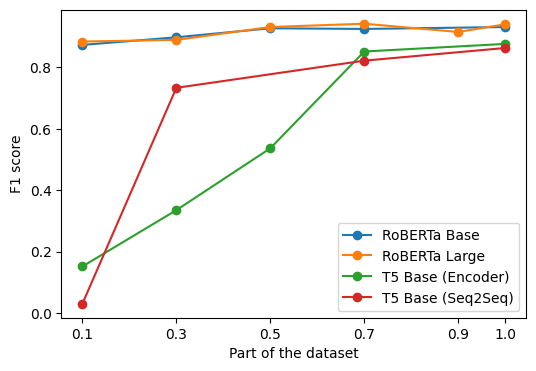
\includegraphics[width=0.63\linewidth]{figs/wos_baseline.png}
    \caption{F1 score performance of baseline models on the WOS dataset across varying dataset sizes.}
    \label{fig:baselines:wos}
\end{figure}
\begin{figure}[p]
    \centering
    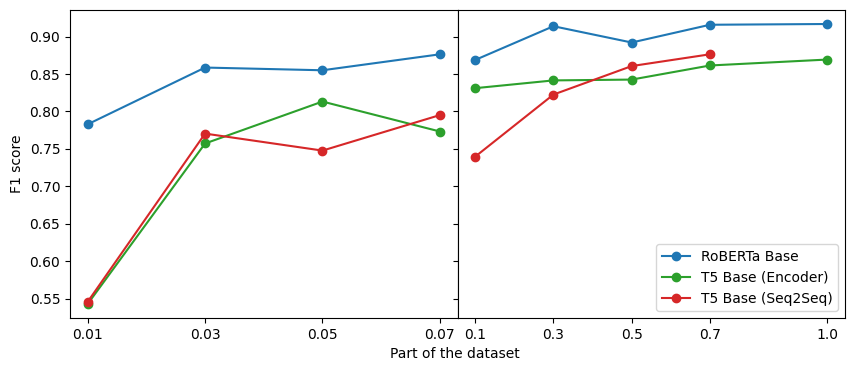
\includegraphics[width=\linewidth]{figs/esnli_baseline.png}
    \caption{F1 score performance of baseline models on the e-SNLI dataset across varying dataset sizes.}
    \label{fig:baselines:esnli}
\end{figure}

These figures vividly illustrate the performance of each model across various dataset sizes, offering a detailed visualization of the models' accuracy and efficiency.

This comprehensive overview allows for a nuanced analysis of how model effectiveness varies with the size of the dataset. RoBERTa models consistently outperformed T5 models, regardless of their setup, across all dataset sizes, demonstrating their superior performance in sequence classification tasks.

Additionally, RoBERTa exhibited less variance across different dataset sizes, indicating more robust and reliable performance. Conversely, the EncT5 model showed little improvement over the T5 Seq2Seq model, suggesting that the architectural modifications did not significantly enhance its classification capabilities.

These insights give rise to the hypothesis that models designed explicitly for classification, like RoBERTa, may be inherently more suitable for student model compared to more generative models like T5.

\newpage

\stepcounter{experiment}
\section{Experiment \theexperiment: Evaluating T5 model with 2 heads}
\label{sec:t5_2heads}

\subsection*{Experimental Setup}

The student model in this experiment employs a modified T5 architecture \cite{t5}, incorporating a dual-head design to enhance its functionality. This adaptation includes the addition of a classification head alongside the existing language modeling head, which is now specifically tasked with generating rationales (\autoref{fig:modified_t5}). The model is trained on a dataset that consists of labeled examples, with its training trajectory significantly informed by the LLM knowledge. But during the prediction phase, the classification head is used to make predictions, while the language modeling head is not utilized.

\begin{figure}[hbt]
    \centering
    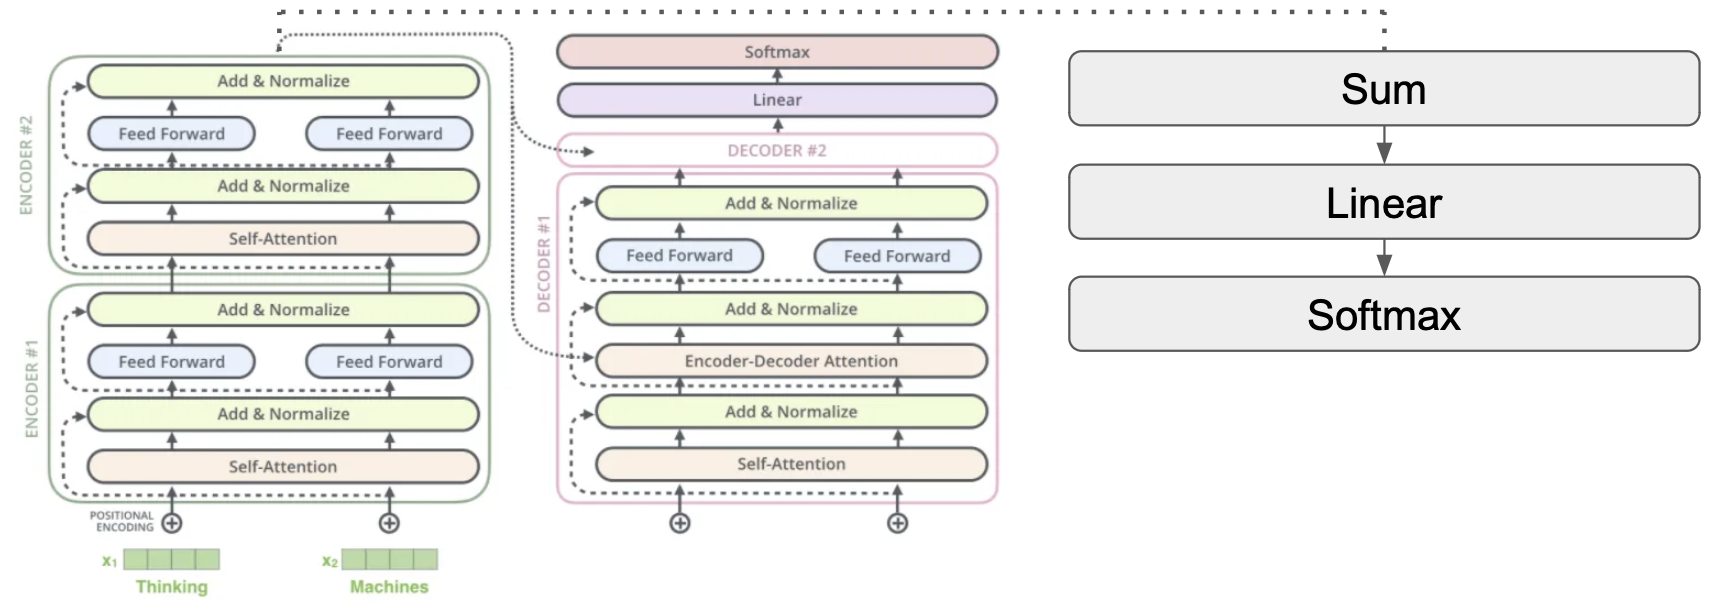
\includegraphics[width=0.99\linewidth]{figs/modified_t5.png}
    \caption{Modified T5 architecture for the student model.}
    \label{fig:modified_t5}
\end{figure}

The use of a linear combination for the loss function optimally balances the contributions from both language modeling and classification tasks during training. Specifically, the combined loss function can be formulated as follows:
$$ L = \alpha L_{LM} + (1 - \alpha) L_{C} $$
Where $L$ represents the total loss, $L_{LM}$ is the original T5 language modeling loss, $L_{C}$ is the classification loss (cross-entropy), and $\alpha$ is a hyperparameter that determines the relative importance of the two losses.

\subsection*{Results}

Irrespective of the selected value for the parameter $\alpha$, there was no observed reduction in the classification loss. Language modeling loss, exhibited some decrease depends on $\alpha$, indicating that the model was learning to generate rationales. This phenomenon may be attributed to the possibility that the features extracted by the T5 encoder, which are utilized by the decoder, are insufficient for the classification task.

% \stepcounter{experiment}
% \section{Experiment \theexperiment: Train T5 Seq2Seq and EncT5 sequentially}

% In this experimental setup, the focus shifts to training the T5 model sequentially for generating rationales and subsequently for classification. This approach aims to evaluate whether a sequential training methodology can enhance the overall performance of the model on sequence classification task.

% The T5 model is initially trained simultaniously on a rationale generation and label generation tasks. The objective during this phase is to train the encoder of the T5 model to understand the context of the dataset explaining ``the nature'' of the dataset.

% Following the rationale generation training, the same T5 model, but without decoder and LM head, undergoes further training on a classification task. During this phase, the classification head is activated, and the model is trained on a dataset of input examples paired with their respective labels.

% This gave an increase in accuracy over EncT5 baseline.

\stepcounter{experiment}
\section{Experiment \theexperiment: Evaluating RoBERTa with rationales}
\label{sec:roberta_rationales}

In this experimental setup, the focus is on leveraging the capabilities of RoBERTa. This experiment investigates whether incorporating rationales directly into the training process of RoBERTa can enhance its understanding and processing of complex input, thereby improving overall performance on classification task.

\subsection*{Experimental Setup}

The RoBERTa model is trained on a dataset of input examples paired with their respective labels. The training process is augmented with the inclusion of rationales generated by the teacher model, sticking to the hypothesis that the model will better understand the training data.

The integration of rationales into the training set is achieved by manipulating the dataset to include both examples with and without rationales. The hypothesis underpinning this experimental setup is that the inclusion of rationales provides a deeper contextual understanding, aiding the model in making more informed decisions during the classification process. By presenting the model with inputs that vary in their contextual richness (with and without rationales), it is possible to directly observe the impact of added context on performance metrics.

\subsection*{Results}

The results of the experiment for the e-SNLI dataset are visualized in the \autoref{fig:roberta_rationales}, which illustrates the F1 score of the RoBERTa model both with and without the inclusion of rationales in the training data.

\begin{figure}[hbt]
    \centering
    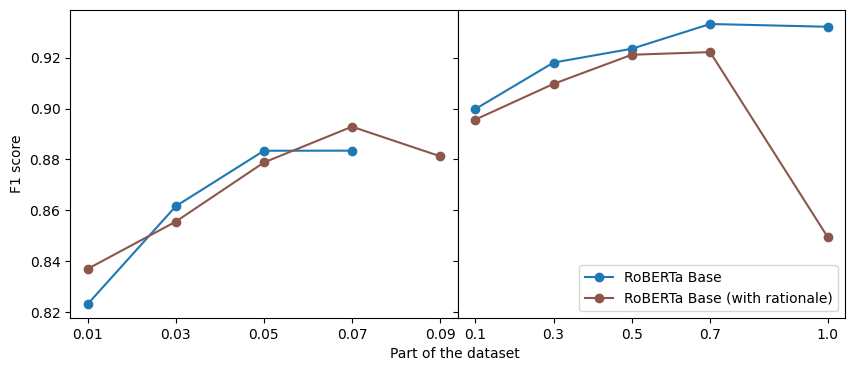
\includegraphics[width=\linewidth]{figs/roberta_rat.png}
    \caption{Results of training RoBERTa with rationales on the e-SNLI dataset.}
    \label{fig:roberta_rationales}
\end{figure}

Despite the theoretical advantages posited by incorporating rationales into the training process, the experiment did not demonstrate a significant increase in metrics over the baseline RoBERTa model, which was trained without the inclusion of rationales. The F1 score, as displayed in the graph, show no improvement, suggesting that the addition of rationales in the manner implemented may not substantially influence the model's ability to classify the input data more effectively.

\stepcounter{experiment}
\section{Experiment \theexperiment: Evaluating Pipeline}

This experiment is designed to evaluate the efficacy of the proposed in \autoref{sec:proposed_method} method, where the T5 model generates rationales and the RoBERTa model performs sequence classification based on these rationales. The experiment aims to demonstrate that this dual-model setup not only enhances classification accuracy but also offers greater interpretability by leveraging the rationales generated by T5.

\subsection*{Experimental Setup}

A specialized dataset splitting is applied for this experiment. The first part of the training dataset is used to train the T5 model to generate rationales that mimic the reasoning provided by the labels, size of this subset is a hyperparameter $\alpha$. The left part of the dataset is used to train the RoBERTa model on the rationales generated by the T5 model.

The T5 model is fine-tuned using the training subset where each input text is associated with a human-generated rationale. This stage aims to train T5 to produce accurate and relevant rationales based on the input text.

After training T5, the generated rationales, along with their corresponding inputs, are used to train the RoBERTa model. This stage focuses on classifying the labels based on the enhanced context provided by the rationales.

The performance of the classification model is assessed using standard metrics described in \autoref{sec:metrics}. Additionally, T5 performance in mimic LLM in generating rationales is evaluated using metrics such as BLEU \cite{bleu}, ROUGE \cite{rouge} and METEOR \cite{meteor}, which measure the textual similarity. But this metrics is used only for eveluation of T5 model, to ensure that it generates rationales that are similar to LLM-generated ones (\autoref{fig:t5_metrics_wos}).

The efficacy of the proposed distillation and classification method is compared against baseline RoBERTa model that classify text without the benefit of rationale generation. This comparison is crucial to demonstrating the added value of incorporating rationale-based learning in the training pipeline.

\subsection*{Results}

The results of the experiment depicted in Fig.\ \ref{fig:pipeline_result:wos} and \ref{fig:pipeline_result:esnli} indicate the performance of the RoBERTa model with and without the integration of the proposed distillation pipeline, measured by the F1 score across different segments of the dataset.

\begin{figure}[p]
    \centering
    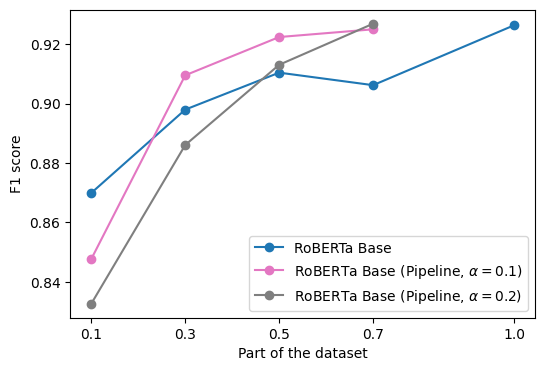
\includegraphics[width=0.63\linewidth]{figs/pipeline_wos.png}
    \caption{F1 score performance of RoBERTa models (baseline and pipeline) on the WOS dataset across varying dataset sizes.}
    \label{fig:pipeline_result:wos}
\end{figure}

\begin{figure}[p]
    \centering
    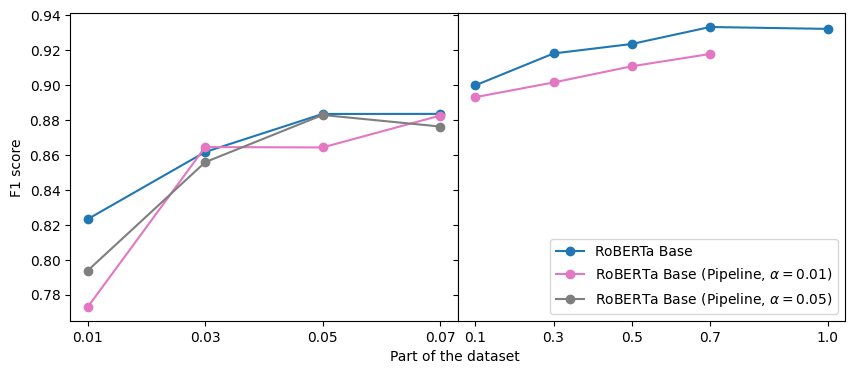
\includegraphics[width=\linewidth]{figs/pipeline_esnli.png}
    \caption{F1 score performance of RoBERTa models (baseline and pipeline) on the e-SNLI dataset across varying dataset sizes.}
    \label{fig:pipeline_result:esnli}
\end{figure}

At the WOS dataset (\autoref{fig:pipeline_result:wos}), the pipeline model with $\alpha = 0.1$ outperformed the baseline model across almost all dataset sizes, excluding the smallest. It demonstres the effectiveness of the proposed method in enhancing classification accuracy. The pipeline model consistently achieved higher F1 scores, indicating that the integration of rationale-based learning into the training process improved the model's classification capabilities.

It seems that the best performance is achieved with a more moderate T5 training set. This might point to the inefficient rationales generated by LLM, for instance, the complexity of the rationales themselves. If the T5 generated rationales are more simplistic or generic, they may provide enough value in helping the classification model (like RoBERTa) to make more informed decisions, but if they are too complex, they may hinder the classification model's performance, like overfitting in classic ML\@.

Incorporating the insights from the e-SNLI dataset's performance highlights the nuanced challenges associated with implementing knowledge distillation techniques in various contexts (\autoref{fig:pipeline_result:esnli}). This result suggests that the effectiveness of the proposed method may be influenced by the complexity and nature of the dataset. Additionaly, leveraging the knowledge embedded within LLM (rationale generation) plays a crucial role in this pipeline. In our case rationales for WOS dataset were more informative than for e-SNLI dataset, which may explain the difference in performance.

The e-SNLI dataset, which is more nuanced and contextually rich, may require additional modifications to the process to achieve optimal performance.

The divergence in performance with different $\alpha$ settings underlines the need for further experimental analysis to understand the interaction between rationale quality, its weighting in the model, and the classification outcomes.

\section{Summary}

This chapter has presented an in-depth examination of multiple experiments conducted to assess the efficacy of knowledge distillation methods in improving sequence classification using LLM as the knowledge source. The results of these experiments provide a comprehensive understanding of how distillation techniques can be leveraged to enhance the performance of smaller models, potentially reshaping training strategies in the NLP field.

The findings suggest that while knowledge distillation and the incorporation of innovative training techniques offer significant potential, the effectiveness of these methods can be highly contingent on the specifics of the task and the dataset. The complexity of the data, the alignment of model capabilities with task requirements, and the quality of the knowledge being distilled are all critical factors that influence the success of distillation strategies.
